\section{Design}

\subsection{ANTLR}
\begin{frame}
\frametitle{ANTLR}

We use ANTLR to generate a parse tree and walk the parse tree to \emph{collect software quality metrics}.

\begin{definition}
ANTLR (ANother Tool for Language Recognition) is a powerful parser generator for reading, processing, executing, or translating structured text or binary files. (Parr, 2013)
\end{definition}

It can \emph{support multiple programming languages}, as long as you define the language structure using a grammar file\footnote{Open source grammar files: https://github.com/antlr/grammars-v4}.

\end{frame}

\subsection{Architecture for Measurement Component}
\begin{frame}
\frametitle{Architecture for Measurement Component}

\only<1>{
  Washizaki et al. (2007) proposed a framework that achieves effective measurement and evaluation of source code quality.

  \begin{center}
  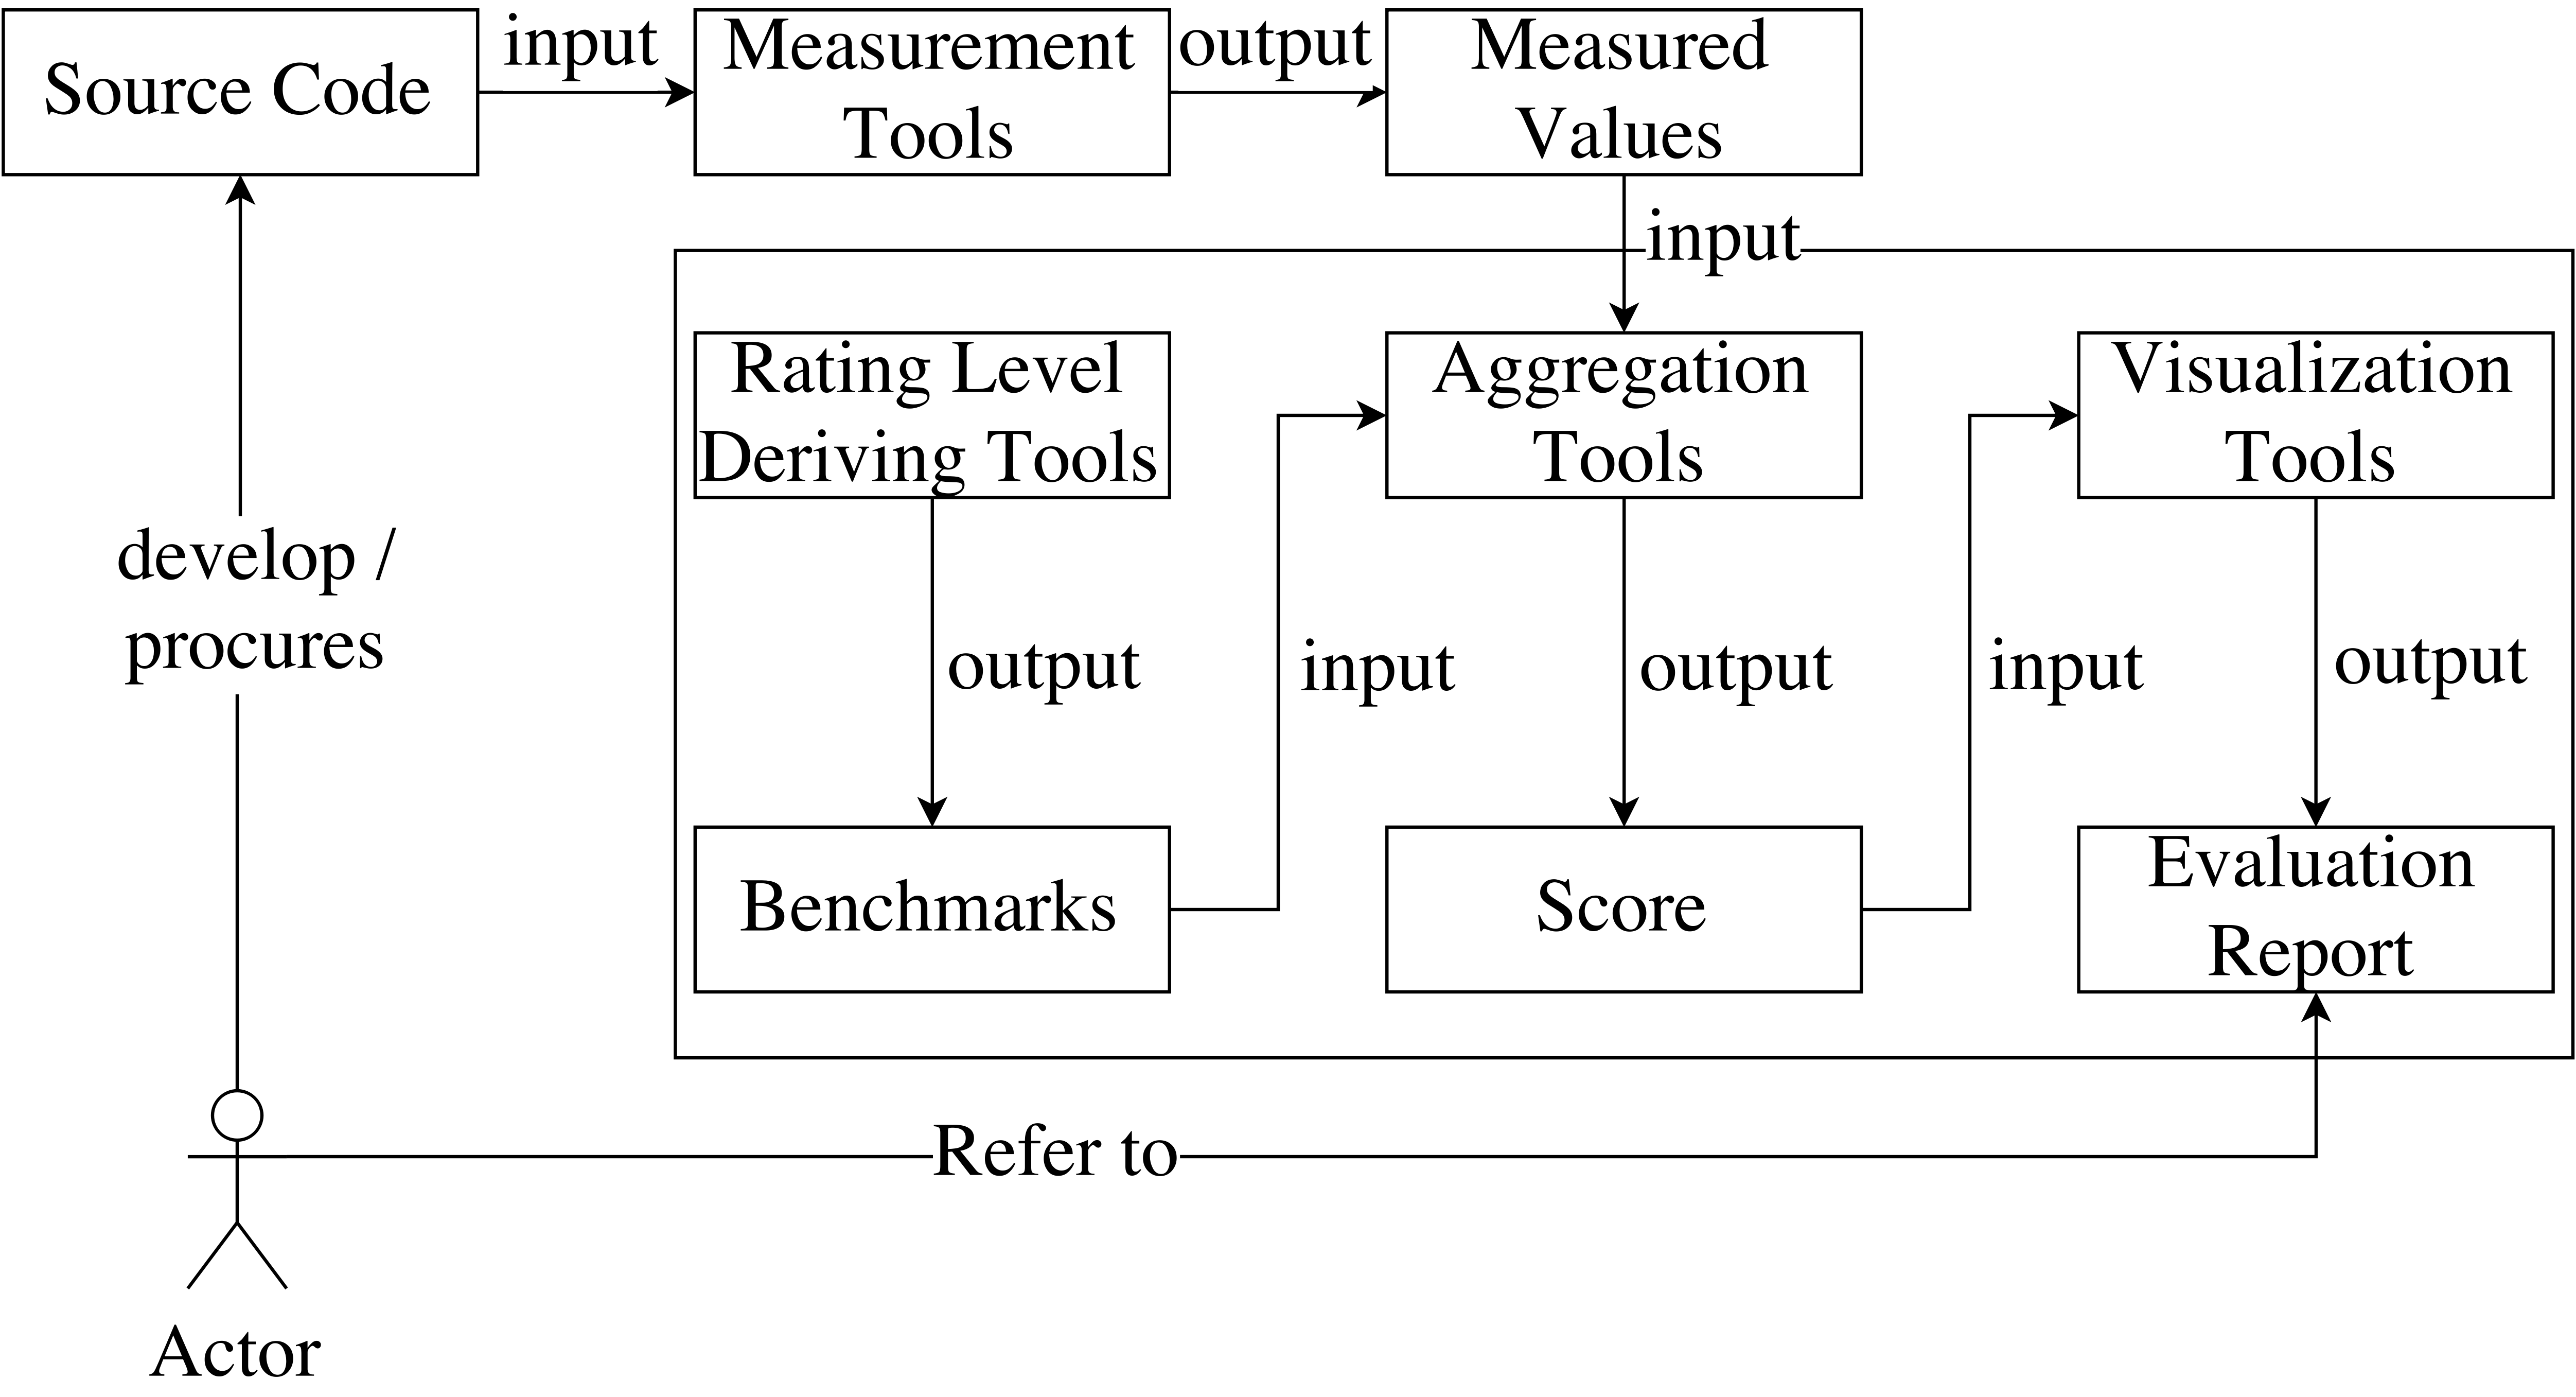
\includegraphics[scale=0.06]{washizaki_framework}
  \end{center}
}

\only<2>{
  We use the proposed framework to build the measurement component of SQAT.

  \begin{center}
  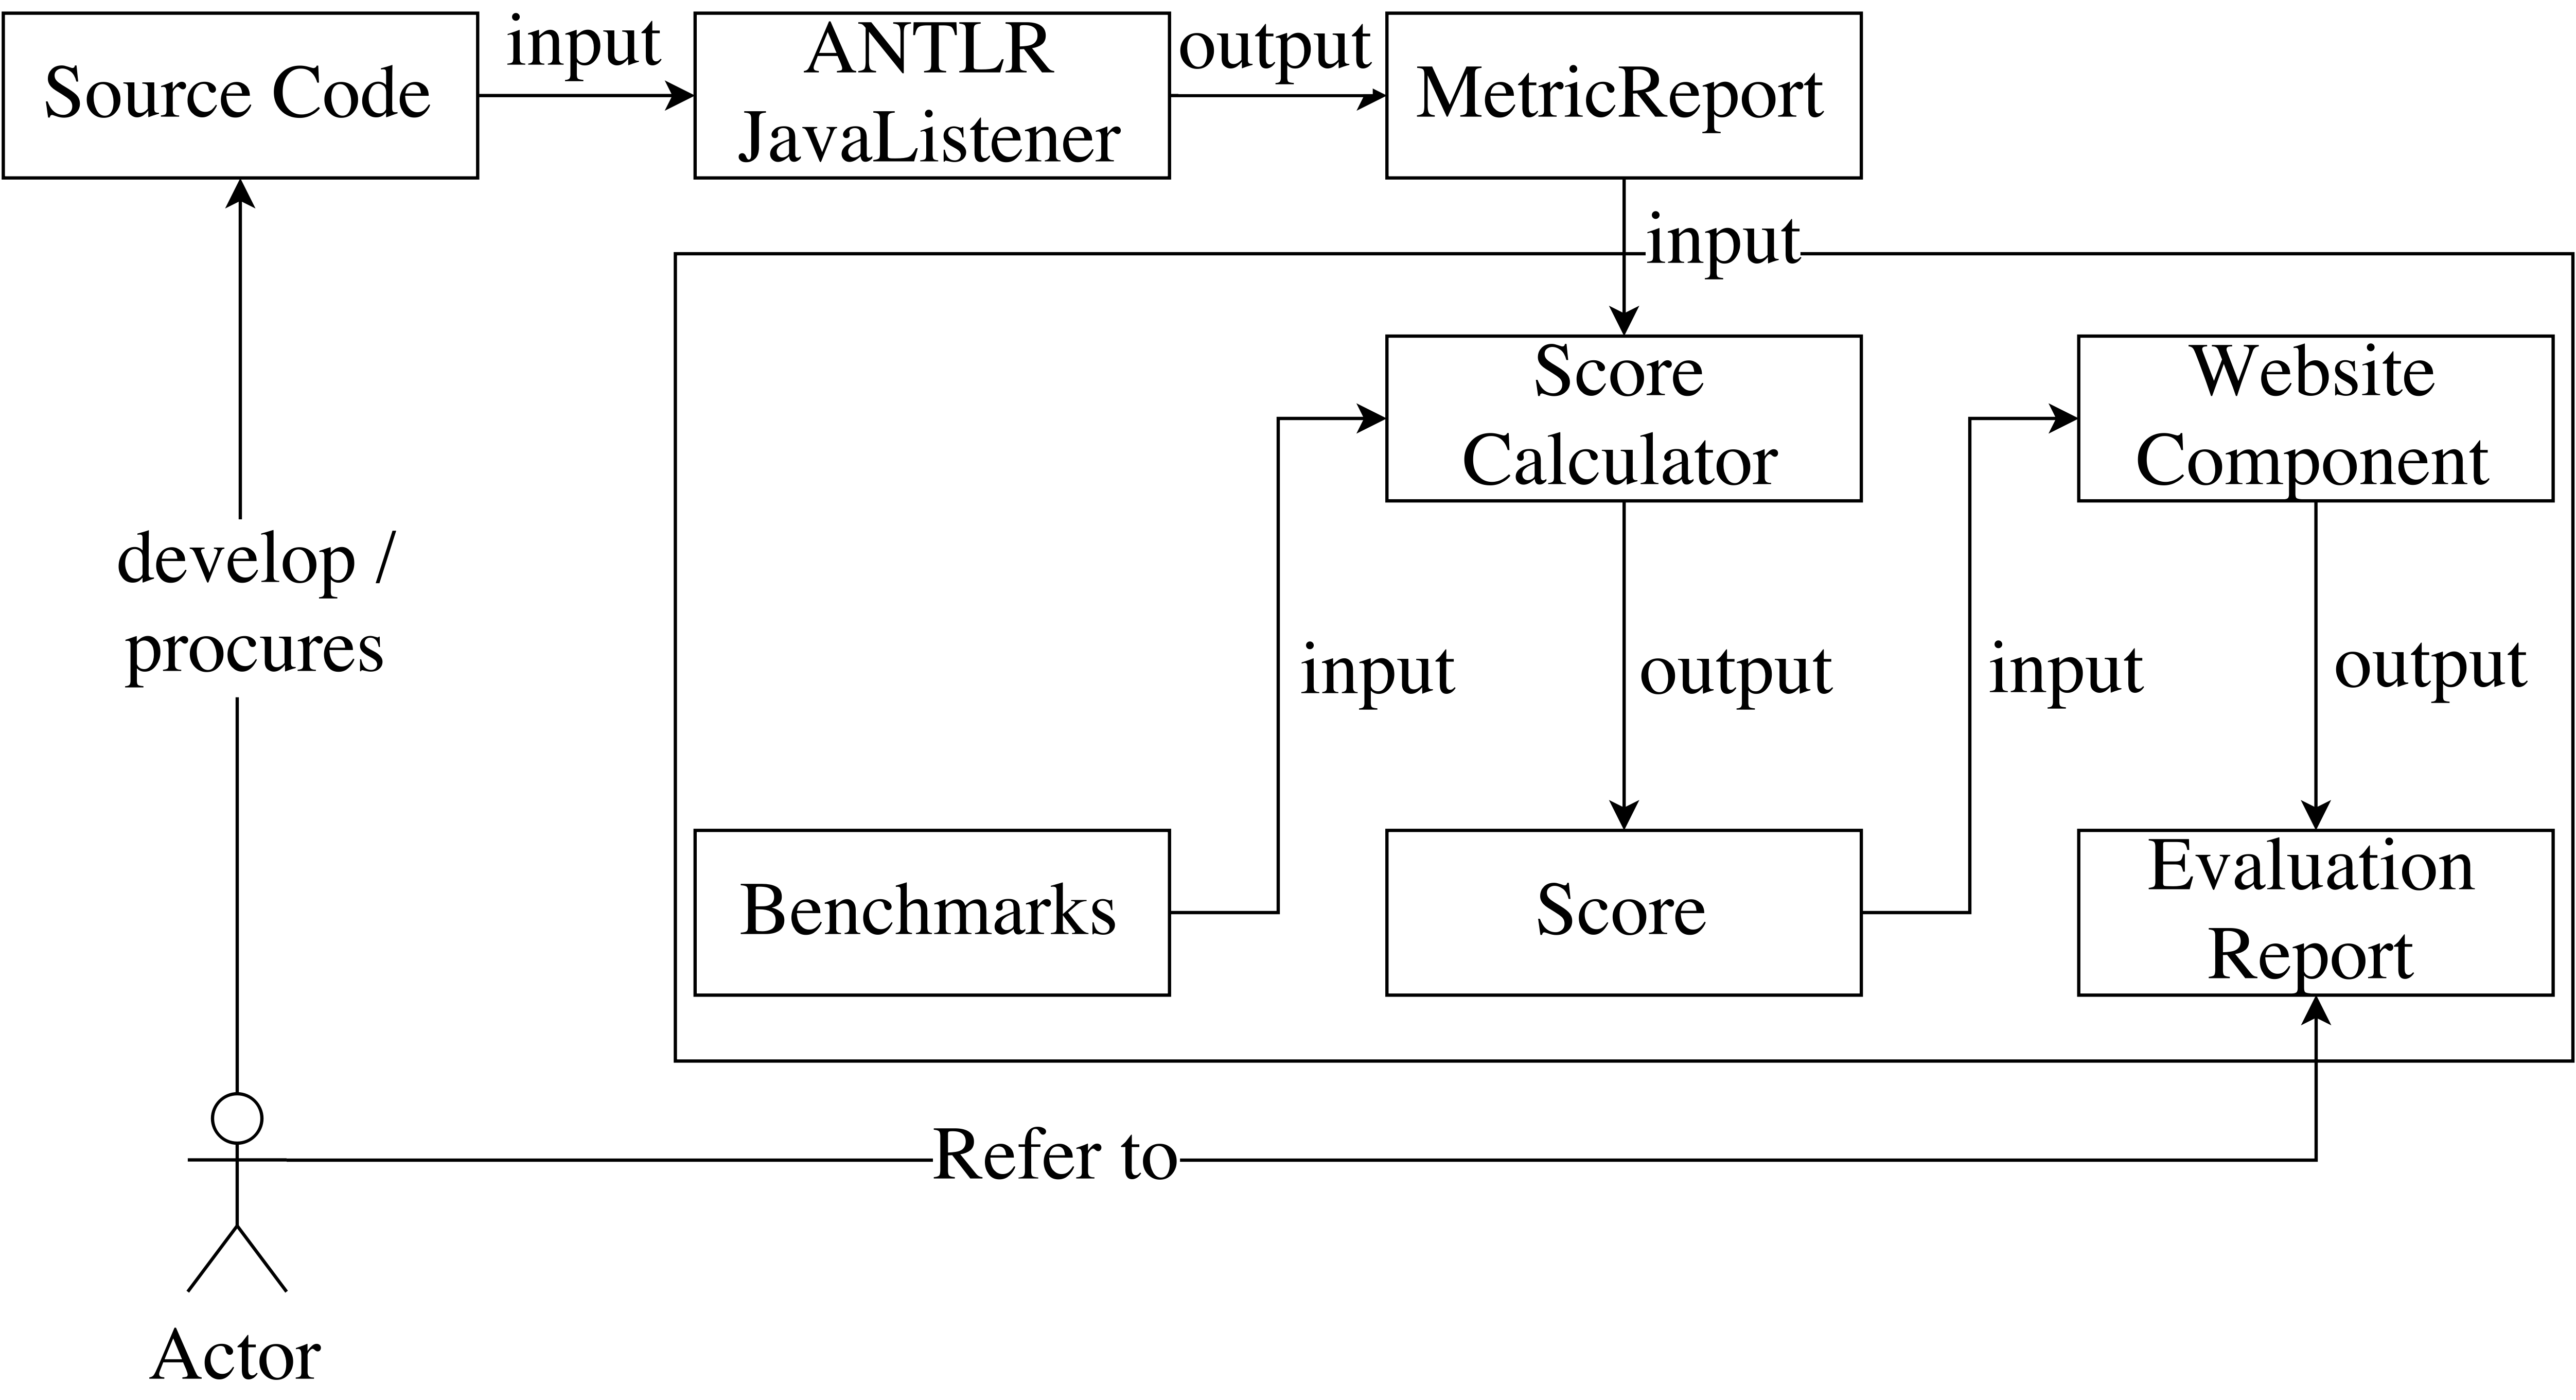
\includegraphics[scale=0.06]{software_quality_measurement_framework}
  \end{center}
}
\end{frame}

\subsection{Overall Architecture}
\begin{frame}
\frametitle{Overall Architecture: Monolithic Architecture}

\only<1,3>{
  \begin{definition}
  Monotolithic architecture is made up of multi-tier components, with components in upper tier use components in lower tier to perform some functions.
  \end{definition}
}

\only<2>{
  \begin{center}
  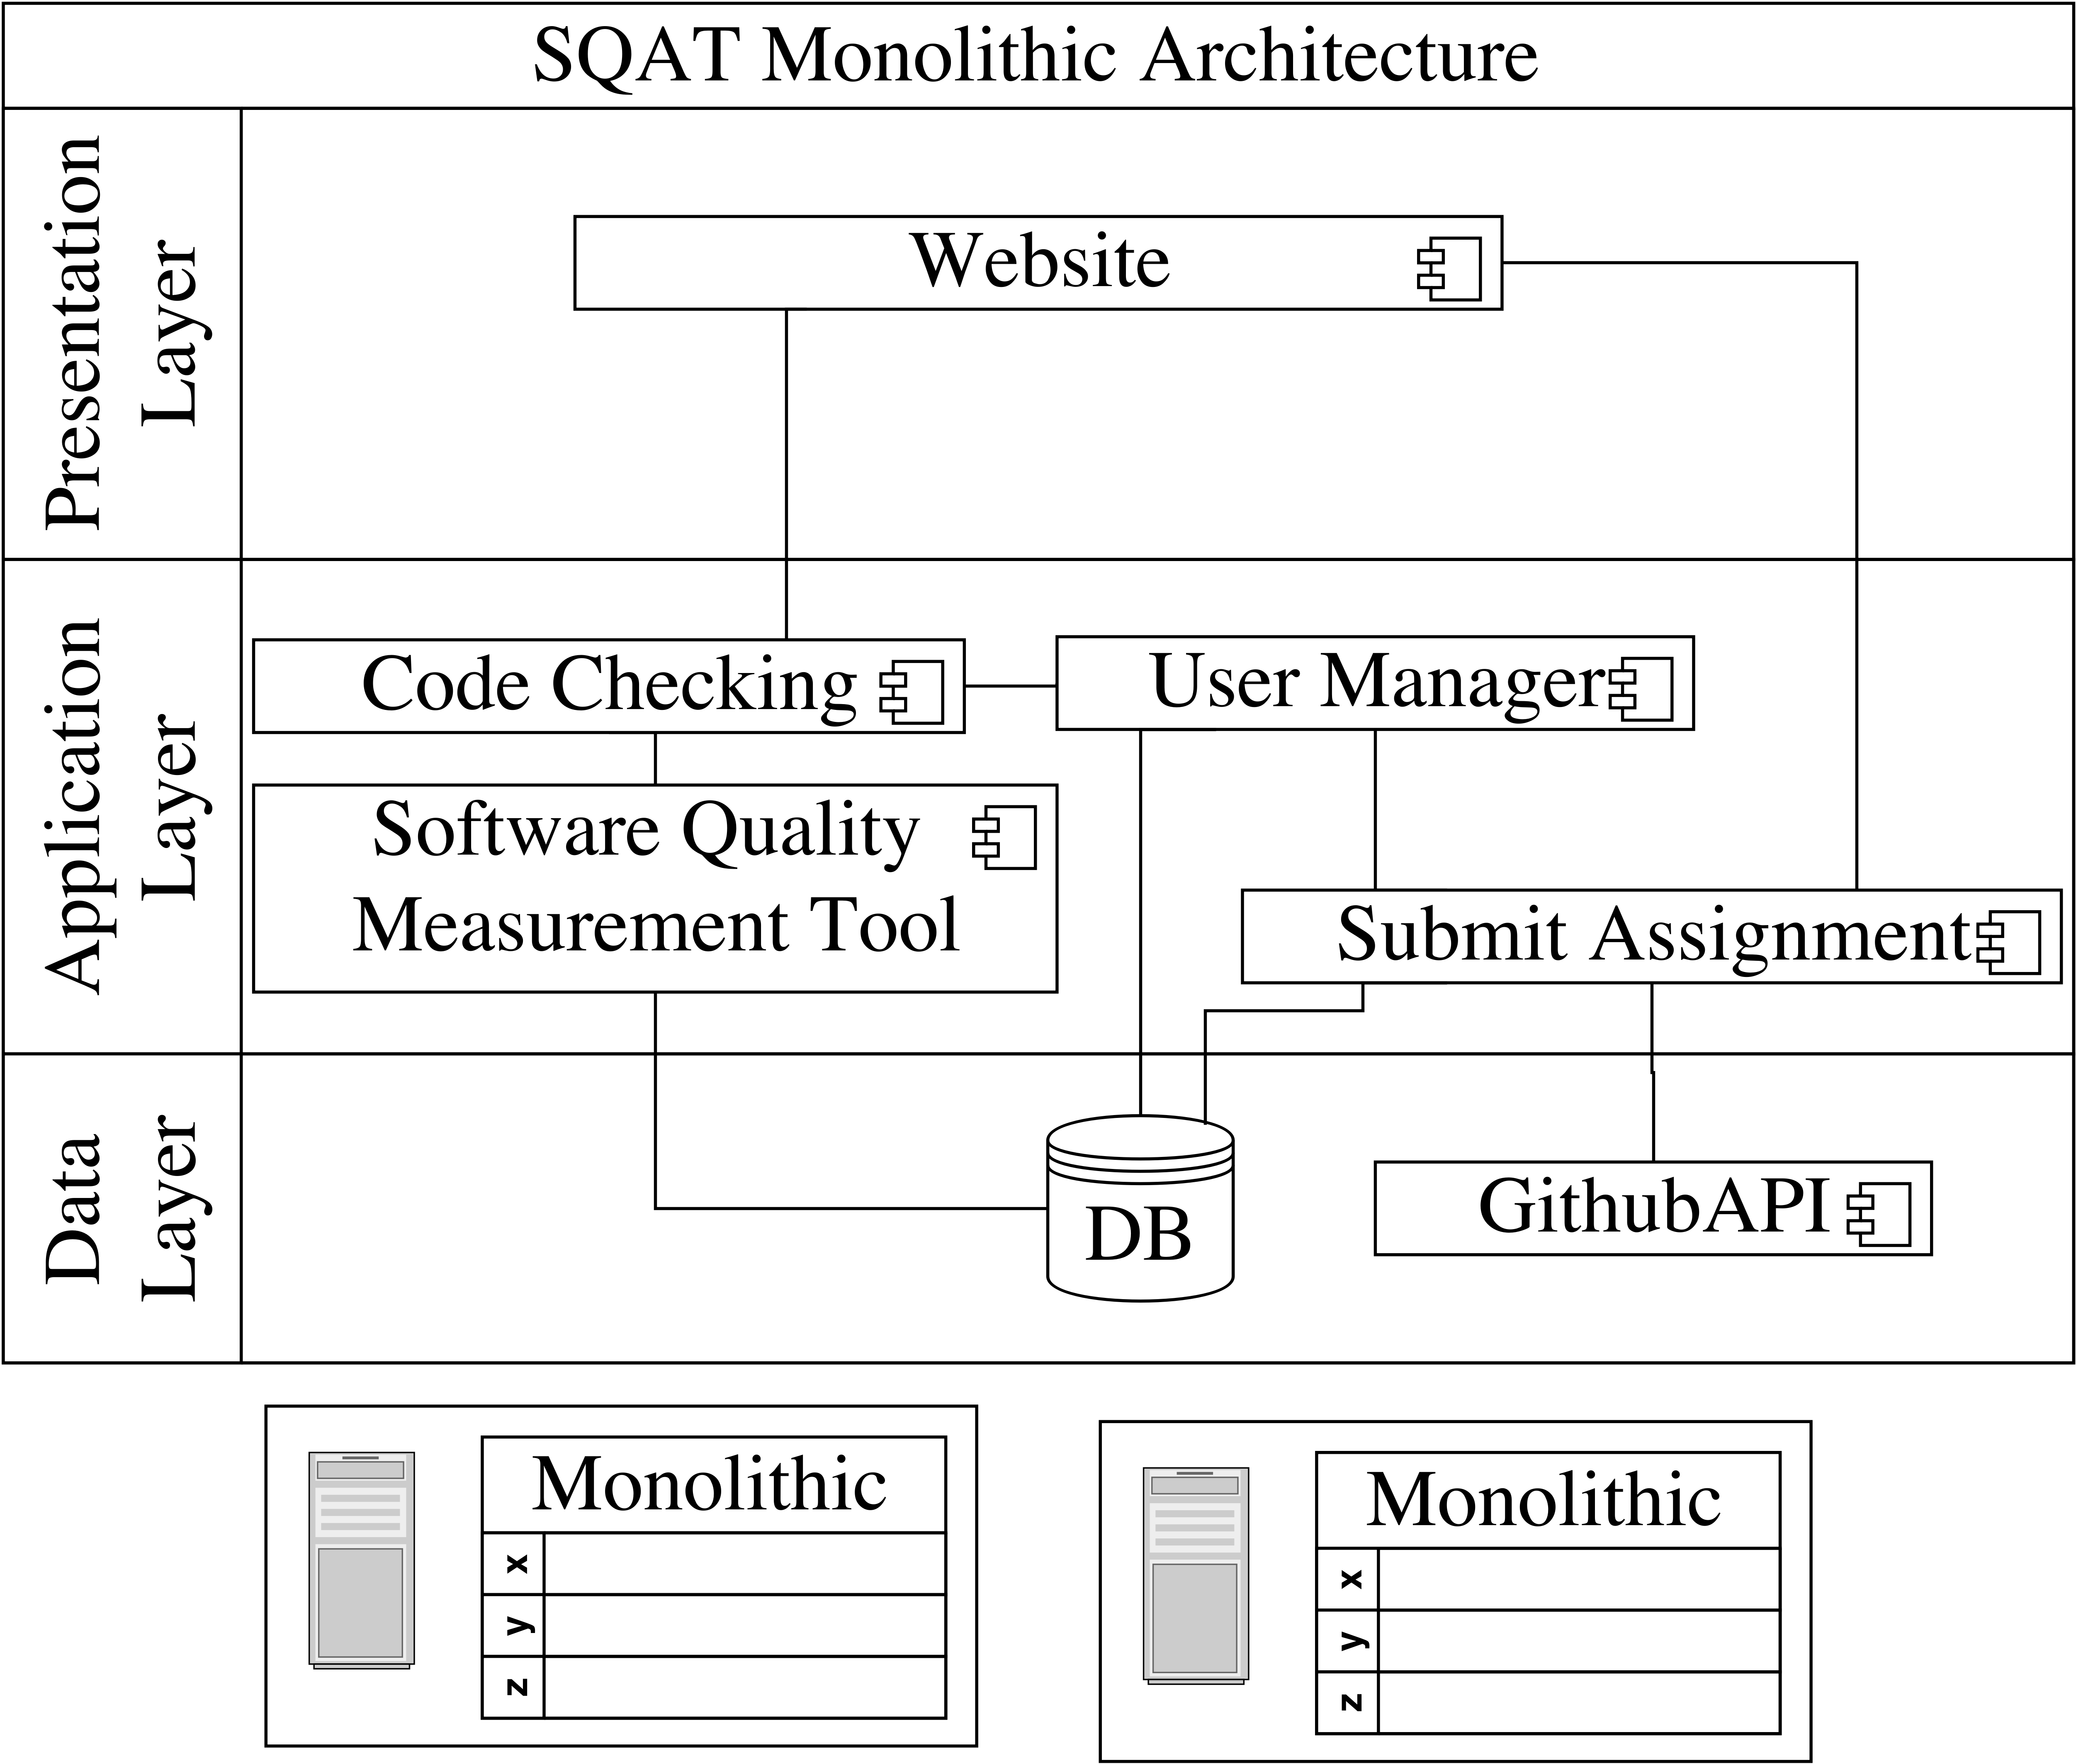
\includegraphics[scale=0.045]{SQAT_monolithic}
  \end{center}
}

\only<3>{
  The architecture has three major drawbacks:
  \begin{itemize}
    \item Requires long-term commitment to a particular technology stack
    \item Difficult for developers to understand the whole application
    \item Difficult to scale an application horizontally
  \end{itemize}
}

\end{frame}

\begin{frame}
\frametitle{Overall Architecture: Microservices}

\only<1,3>{
  \begin{definition}
  Microservices is a software architecture style in which complex applications are composed of small, independent processes communicating with each other using language-agnostic API (Fowler, 2014).
  \end{definition}
}

\only<2>{
  \begin{center}
  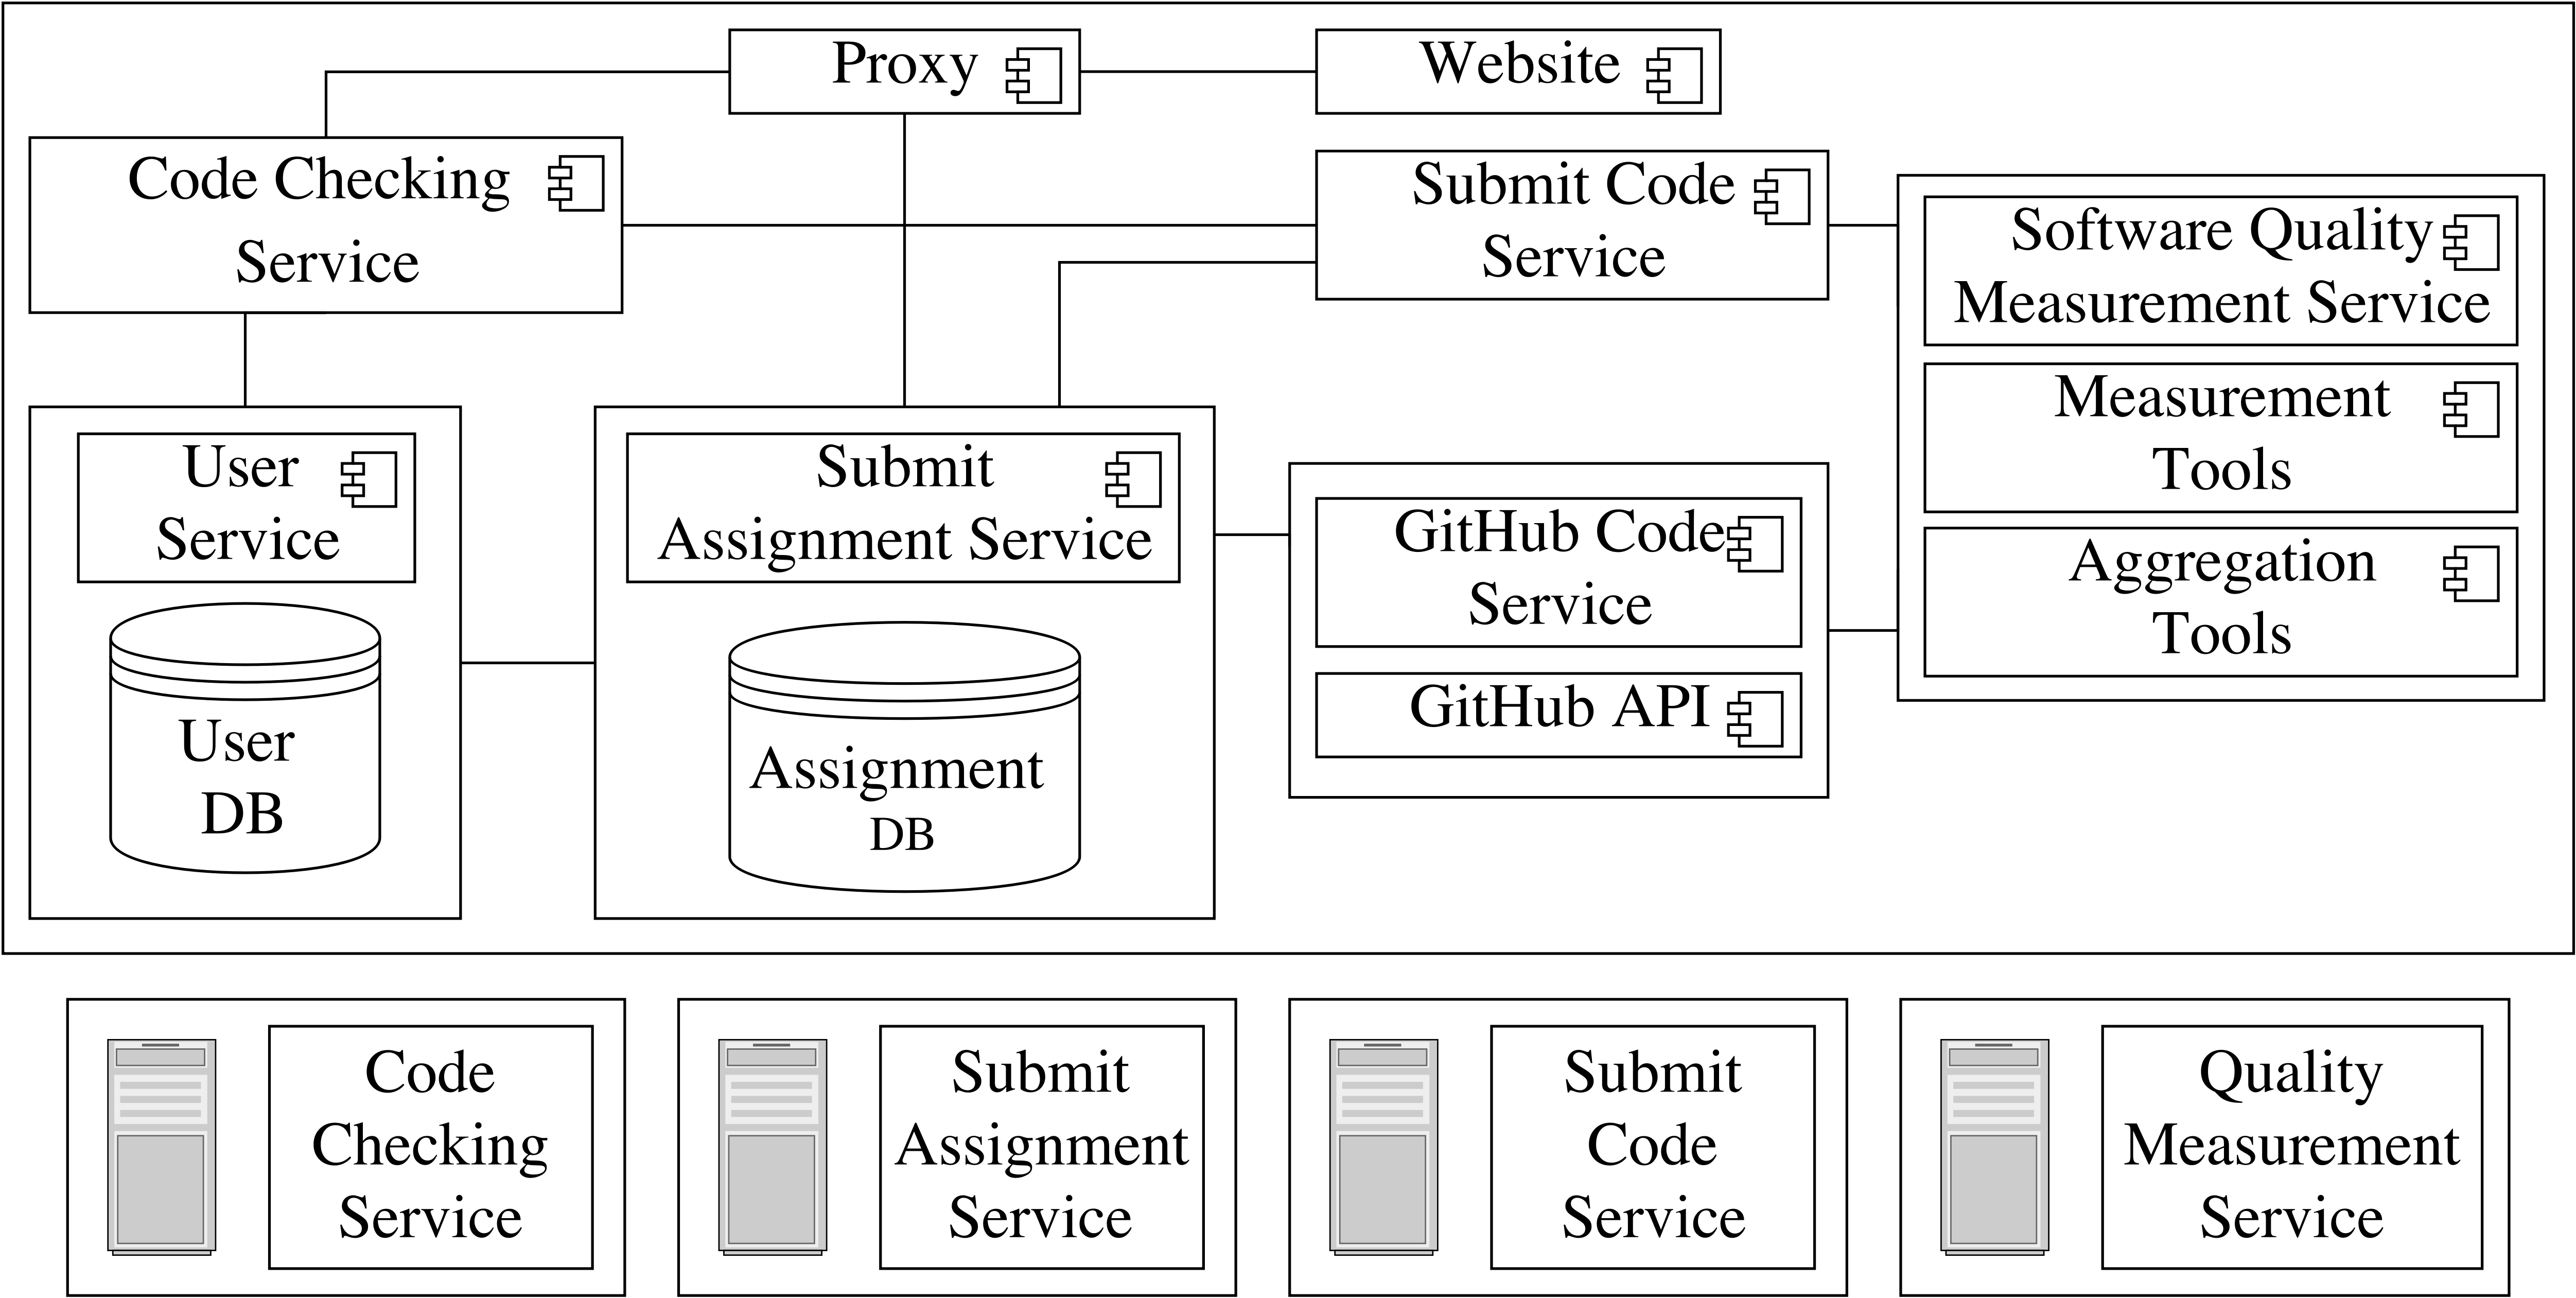
\includegraphics[scale=0.06]{microservice_architecture}
  \end{center}
}

\only<3>{
  The architecture has three advantages:
  \begin{itemize}
    \item Programming language agnostic
    \item Easy to understand due to abstraction at service level
    \item Easy to scale application horizontally
  \end{itemize}
  We use microservices to develop SQAT.
}

\end{frame}